\section{Постановка задачи}

\subsection{Введение}
\subsubsection{Цель и назначение разработки}

Цель разработки – разобраться со структурой интерпретатора современного языка программирования.

Назначение разработки – синтаксический разбор, проверка типов (семантический анализ), нормализация посредством вычисления, вывод в консоль.

\subsubsection{Область применения}

Прямой области применения у разработки нет. Несмотря на это, почти все из статически-типизированных языков программирования, применяющихся в индустрии, можно свести к просто-типизированному лямбда-исчислению, что указывает на широкую применимость этого формализма и следовательно, применимость разработки. Разработку планируется постепенно расширить более реалистичными особенностями с целью получения корректного интерпретатора для какой-либо конкретной области.

\subsubsection{Определения, термины, сокращения}

\begin{description}
  \item{ЛИ} Лямбда-исчисление
  \item{ТТ} Теория типов
  \item{ПО} Программное обеспечение
\end{description}

\subsection{Общее описание}

Название проекта - "Типизированный интерпретатор просто-типизированного $\lambda$-исчисления".

В настоящий момент разного рода интерпретацией занимается очень большое количество программ и библиотек (начиная от графических, например, Cairo, и заканчивая системными, например, printf в POSIX). Вследствие этого возникла потребность в изучении и разработке более эффективных способов построения интерпретаторов.

В этих условиях интерпретаторы становятся важным элементом инструментария.

В настоящее время на казахстанском рынке никто не занимается производством интерпретаторов.

Таким образом, актуальными являются исследования, направленные на разработку интерпретаторов с целью их практической реализации. 

Главной задачей является написание интерпретатора, состоящего из проверки типов и вычислителя.

\subsubsection{Пользовательские интерфейсы}

Интерфейсом программы является текстовый терминал.

\subsubsection{Аппаратные интерфейсы}

Требования к оборудованию, на котором будет работать интерпретатор:
 
Частота процессора --- 1 GHz, оперативная память --- 128 Мб, место на жёстком диске --- 2 Mb.

\subsubsection{Программные интерфейсы}

Требования к установленному на серверной стороне программному обеспечению:

Операционная система – Linux, *BSD, GCC версии 4.2 или выше, ATS/Anairiats версии 0.2.0 или выше.

\subsubsection{Коммуникационные интерфейсы}

Требований к коммуникационным средствам не предъявляется.

\subsubsection{Требования по адаптации}

Текстовый интерфейс интерпретатора должен поддерживать работы с любыми версиями популярных эмуляторов терминалов. 

\subsection{Требования к разработке}
\subsubsection{Функциональные требования}
\subsubsection{Требования к функциональным характеристикам}

Функции, выполнение которых должна обеспечивать система: 

\begin{itemize}
\item Открытие файла-скрипта;
\item Ввод новых данных из командной строки;
\item Вывод результатов вычисления в командную строку;
\item Лексический анализ и минимальные сообщения об ошибках;
\item Проверка типов и минимальные сообщения об ошибках.
\end{itemize}

\subsubsection{Исходные данные}

Исходными данными в этой системе будут являться заготовленные заранее файлы с программами в текстовом представлении. Синтаксически формат строго фиксированный, и определён контекстно-свободной грамматикой с помощью нормальной формы Бэкуса. Расширение файла программы – *.stlc.

Ниже представлена одна из программ:

\begin{lstlisting}
\x:int->int.\y:int.(x y):int
\end{lstlisting}

\subsubsection{Результаты}

Цель вычисления – найти нормальную форму лямбда-терма посредством редукций.

\subsubsection{Формат выходных данных}

Результатом вычисления должен быть лямбда-терм в нормальной форме.

\subsubsection{Организация функциональных требований}
\subsubsection{Организация требований по диаграммам потоков данных}

\subsection{Нефункциональные требования}
\subsubsection{Производительность}

Строгих требований к производительности системы и потреблению памяти не предъявлялось, так как разработка является экспериментальной. Несмотря на это, использование асимпототически эффективных алгоритмов рекомендуется.

\subsubsection{Надёжность и доступность}

Эта система надежна и формально верифицирована на соответствии частичной спецификации, выраженной посредством системы типов ATS (при условии, что все нижележащие уровни, т.е. стандартная библиотека, ОС и аппаратура, работают корректно).

\subsubsection{Обработка ошибок}

Вследствие того, что целью разработки не было создание интерпретатора промышленного качества, сообщения об ошибках при синтаксическом и семантическом анализах не очень удобны пользователю.

\subsubsection{Интерфейсные требования}

Единственными элементами интерфейса самого интерпретатора является одно окно, в котором отображается ход интерпретации. Окно изображено на рис. \ref{example}.

\begin{figure}
\center{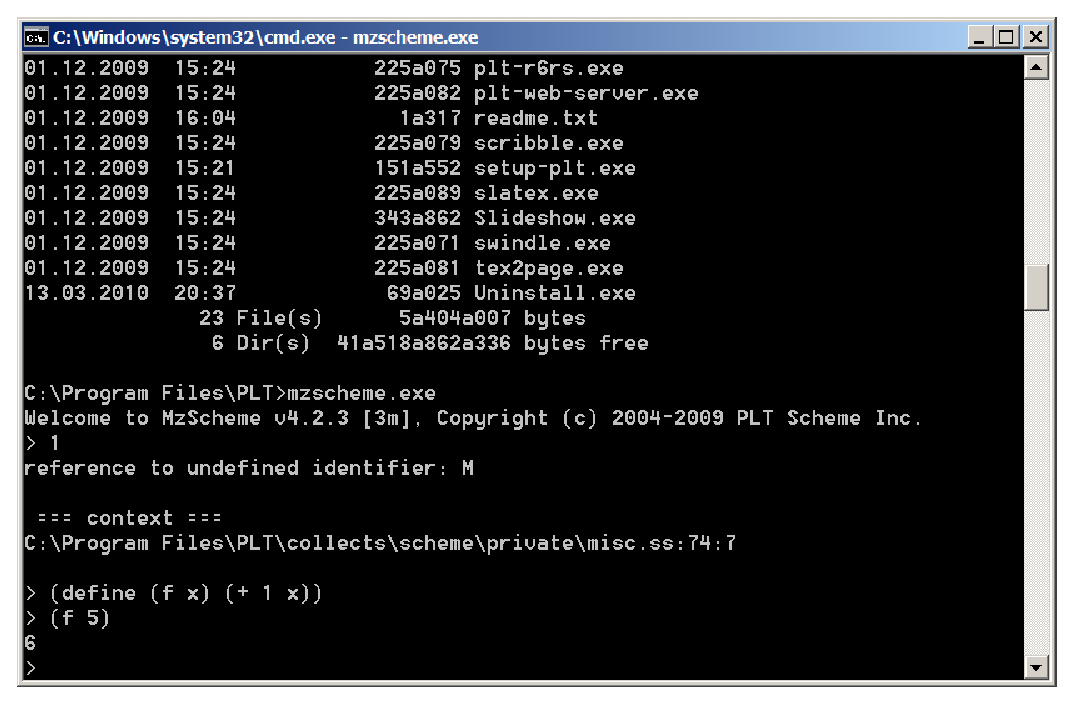
\includegraphics[width=0.75\linewidth]{racket}}
\caption{Пример внешнего вида приложения}
\label{example}
\end{figure}

\subsubsection{Ограничения}

Точность выходных данных должна быть таковой, чтобы математик, проверив шаги выполнения, мог с твердостью заявить, что результат корректен. То есть, результат должен быть однозначно правильным.

Система должна быть разработана на языке программирования ATS, потому что сходные инструменты (такие, как Haskell и OCaml) не предоставляют такой же выразительной системы типов.

Язык возможного интерфейса – английский. Стиль – строгий, технический.

К разработке системы не должны привлекаться третьи лица.

\subsection{Обратные требования}

Система не будет автоматически писать программы – это должен сделать специалист зoаранее.

Система не будет описывать процесс редукции по шагам. Она лишь вычислит нормальную форму для последующего анализа специалистом.

Система не будет исправлять синтаксические или семантические ошибки автоматически – она лишь укажет на их существование.
o
\section{Практическая часть}

\subsection{Просто-типизированное $\lambda$-исчисление}
\label{sec:stlc}

\emph{Тип} является коллекцией вычислительных сущностей, которые имеют некоторые общие свойства. Например, тип $int$ назначается всем выражениям, результатом вычисления которых будет целое число, а тип $int \implies int$ назначается всем функциям от целых к целым.

Типы можно рассматривать как ёмкие, приблизительные описания вычислений: типы являются \emph{статической} аппроксимацией поведения программы при выполнении. Системы типов являются легковесным формальным методом для размышления о поведении программ.

\subsubsection{Синтаксис}

Синтаксис просто-типизированного $\lambda$-исчисления подобен синтаксису бестипового $\lambda$-исчисления за исключением абстракций. В абстракции $\lambda x: \tau . e$ тип $\tau$ является ожидаемым типом аргумента $x$.

Термы, находящиеся в нормальной форме, выделены в отдельную категорию \emph{значений}.

\begin{center}
$e$ ::= $x \in V$ | $\lambda x : \tau. e$ | $e_1 e_2$ | $n$ \\
$v$ ::= $\lambda x : \tau. e$ | $n$ \\
$\tau$ ::= int | $\tau_1 \implies \tau_2$
\end{center}

\subsubsection{Отношение типизации}

Присутствие типов не изменяет способ вычисления лямбда-выражений, отношение редукции определяется по аналогии с бестиповым $\lambda$-исчислением.

Типы используются для ограничения множества вычисляемых выражений. Система типов просто-типизированного $\lambda$-исчисления позволяет удостовериться, что вычисление любой программы, прошедшей проверку типов, не зайдет в тупик. Вычисление выражения $e$ называют \emph{зашедшим в тупик}, если $e$ не является значением, но его невозможно редуцировать до $e_1$.

Отношение между выражениями и типами $\Gamma \vdash e:\tau$ читается как <<выражение $e$ имеет тип $\tau$ в контексте $\Gamma$. Типовый контекст является списком переменных и их типов. В умозаключении $\Gamma \vdash e:\tau$ все свободные переменные $e$ связаны с типами в контексте $\Gamma$.

Формально, типовый контекст определяется как
\begin{center}
$\Gamma$ ::= $\emptyset$ | $\Gamma, x:\tau$
\end{center}

Пусть даны контекст $\Gamma$ и выражение $e$. Если существует некоторый тип $\tau$, такой, что $\Gamma \vdash e:\tau$, говорят, что \emph{$e$ присваивается тип $\tau$ в контексте $\Gamma$}.

Отношение $\Gamma \vdash e:\tau$ определяется индуктивно посредством следующих правил.

$$
\infer[(var)]{\Gamma \vdash x:\tau}{\Gamma (x) = \tau}
\qquad \infer[(int)]{\Gamma \vdash n:int}{}
\qquad \infer[(abst)]
  {\Gamma \vdash \lambda x:\tau_1 . e : \tau_1 \implies \tau_2}
  {\Gamma,x:\tau_1 \vdash e:\tau_2}
$$
$$
\infer[(app)]
  {\Gamma \vdash e_1 e_2 : \tau_2}
  {\Gamma \vdash e_1:\tau_1 \implies \tau_2 & \Gamma \vdash e_2:\tau_1}
$$

Целому числу всегда назначается тип $int$. Переменная $x$ имеет, с которым она связана в контексте (разумеется, контекст должен содержать $x$). Абстракция $\lambda x: \tau_1 . e$ имеет тип $\tau_1 \implies \tau_2$ если выражение $e$ имеет тип $\tau_2$ при условии, что $x$ имеет тип $\tau_1$. И наконец, аппликация $e_1 e_2$ имеет тип $\tau_2$, если $e_1$ имеет тип $\tau_1 \implies \tau_2$, а $e_2$ имеет тип $\tau_1$.

Проверка типов позволяет удостовериться, что если программе может быть присвоен тип, то она не <<застрянет>> при выполнении. Это свойство можно описать более формально:
\begin{description}
  \item[Обоснованность] Если $\vdash e:\tau$ и $e \overset{\ast}{\Rightarrow} e'$, то либо $e'$ является значением, либо существует такое $e''$, что $e' \overset{\ast}{\Rightarrow} e''$.
\end{description}

Обычно эту теорему доказывают при помощи двух лемм: о \emph{сохранении} и о \emph{прогрессе}. Лемма о сохранении гласит, что если выражение $e$ назначен тип, и его можно редуцировать или $\alpha$-конвертировать в $e'$, то $e'$ тоже будет назначен тип. Иными словами, редукция сохраняет типизацию. Лемма о прогрессе гласит, что если выражению $e$ назначен тип, то либо это значение, либо существует такое $e'$, что $e \Rightarrow e'$.

Обе леммы можно записать более формально:
\begin{description}
\item[Сохранение] Если $\vdash e:\tau$ и $e \Rightarrow e'$, то $\vdash e':\tau$.
\item[Прогресс] Если $\vdash e:\tau$, то либо $e$ является значением, либо $e \Rightarrow e'$
\end{description}

Из соображений экономии места доказательства теорем, а также многие другие вопросы не раскрываются. Более подробное изложение можно найти в \cite{barendregt1992lambda}.

\subsubsection{Операционная семантика}
%\label{sec:interp}

Операционная семантика позволяет указать смысл программы путем описания того, какие шаги интерпретации необходимо предпринять для вычисления результата. Эти шаги называются \emph{семантикой} программы.

Структурная операционная семантика была предложения Г. Плоткиным в \cite{plotkin1981structural}. Основной идеей является определение поведения программы в терминах поведения ее частей, то есть на основе синтаксиса, отсюда название. Спецификация семантики принимает форму правил вывода.

Правила показывают отношение между выражением и результатом его вычисления. <<$e$ вычисляется в $v$>> пишут $e \Downarrow v$.
$$
\infer[(evalint)]
  {i:int \Downarrow i:int}{}
\qquad
\infer[(evallam)]
  {\lambda x:\tau.e \Downarrow \lambda x:\tau.e}{}
$$
$$
\infer[(evalapp)]
  {e_1 e_2 \Downarrow [v/x]e: \tau_2}{e_1 \Downarrow \lambda x: \tau_1.e:\tau_1 \Rightarrow \tau_2 & e_2 \Downarrow v: \tau_1}
$$

Правила $(evalint)$ и $(evallam)$ показывают, что результатом вычисления функций и целых чисел являются они сами. Согласно правилу $(evalapp)$, вычисление применения функции к аргументу вовлекает в себя вычисление выражения для получения функции, затем вычисление аргумента, и наконец, подстановку.

\subsection{Типизированное внутреннее представление}

Синтаксис для просто-типизированного $\lambda$-исчисления определяется также, как и в предыдущем разделе.

Вместо того, что представлять $\lambda$-выражения, не содержащие сведения о типах, напрямую, предлагается представлять типовую деривацию $\lambda$-выражения. С этой целью определяется суждение $\Gamma \vdash_0 x:\tau$ со смыслом <<$x$ назначен тип $\tau$ в контексте $\Gamma$>>. Правила вывода этого суждения указаны ниже:

$$
\infer[(varZ)]{\Gamma, x:\tau \vdash_0 x:\tau}{}
\qquad \infer[(varS)]{\Gamma, x':\tau_2 \vdash_0 x:\tau_1}{\Gamma \vdash_0 x:\tau_1}
$$

Правило $(var)$ теперь можно изменить:
$$
\infer[(var)]{\Gamma \vdash x:\tau}{\Gamma \vdash_0 x:\tau}
$$

Абстрактный синтаксис представлен ниже.

\begin{lstlisting}[basicstyle=\small]
datasort tp = tpint | tpfun of (tp, tp)
datasort tps = tpsnil | tpsmore of (tps, tp)
\end{lstlisting}

Для представления типов и контекста просто-типизированного $\lambda$-исчисления используются типовые индексы $tp$ и $tps$, соответственно. Например,
\begin{lstlisting}
tpsmore (tpsmore (tpsnil, tpfun (tpint, tpint)), tpint)
\end{lstlisting}
представляет контекст, в котором первой и второй переменной назначены типы \lstinline!tpint! и \lstinline!tpfun (tpint, tpint)!. В целом, контекст $\Gamma = \emptyset, x_1:\tau_1, \ldots, x_n:\tau_n$ представляют в виде \lstinline!tpsmore (\ldots tpsmore (tpsnil, t_n) \ldots, t_1)!, предполагая, что \lstinline!t_i! соответствует $\tau_i$ для любого $1 \leq i \leq n$.

Теперь можно объявить зависимые типы данных для представления типовых дериваций выражений просто-типизированного $\lambda$-исчисления:

\begin{lstlisting}
dataprop TPI (int, T:tp, G:tps) =
  | TPIone (0, T, tpsmore (G, T))
  | {T2:tp} {n:nat} TPIshi (n+1, T, tpsmore (G, T2))
      of TPI (n, T, G)

datatype EXP (G:tps, T:tp) =
  | {n:nat} EXPvar (G, T) of (TPI (n, T, G) | int n)
  | {T':tp} EXPlam (G, tpfun (T, T')) of EXP (tpsmore (G, T), T')
  | {T':tp} EXPapp (G, T') of (EXP (G, tpfun (T, T')), EXP (G, T))
\end{lstlisting}

Фигурные скобки используются для обозначения универсальной квантификации. Конструктор \lstinline!TPI! принимает типовый индекс $i$ сорта $nat$, типовый индекс $G$ сорта $tps$, типовый индекс $T$ сорта $tp$ и формирует тип высказываний \lstinline!TPI (i, T, G)! для представления дериваций $\Gamma \vdash_0 x:\tau$, где $G$ и $T$ представляют $\Gamma$ и $\tau$, соответственно.

Следует заметить, что \lstinline!TPIone! и \lstinline!TPIshi! соответствуют двум правилам типизации, $(varZ)$ и $(varS)$, соответственно. По сути, переменные закодированы индексами Де Брауна: \lstinline!TPIone! является индексом 0 и указывает на первую переменную в контекста, а \lstinline!TPIshi! является оператором сдвига, который увеличивает индекс на единицу. К примеру, \lstinline!TPIshi (TPIshi (TPIone ()))! представляет индекс 3, указывающий на третью по счету переменную в контексте.

Как и \lstinline!TPI!, конструктор типа \lstinline!EXP! также принимает типовой индекс \lstinline!G! сорта $tps$ и типовой индекс \lstinline!T! сорта $tp$, формируя тип \lstinline!EXP (G, T)! для значений, представляющих типовые деривации $\Gamma \vdash e:\tau$, где \lstinline!G! и \lstinline!T! представляют $\Gamma$ и  $\tau$, соответственно.

Конструкторы данных \lstinline!EXPvar!, \lstinline!EXPlam!, \lstinline!EXPapp! соответствуют правилам типизации $(var)$, $(lam)$, $(app)$, соответственно.

Таким образом формируется типизированное внутреннее представление для просто-типизированного $\lambda$-исчисления, и тип объектного языка отражается в типе мета-языка. Между типовой деривацией $\Gamma \vdash e:\tau$ и значением типа \lstinline!EXP(G,T)!, где \lstinline!G! и \lstinline!T! представляют $\Gamma$ и $\tau$, соответственно.

Просто-типизированное $\lambda$-исчисление можно расширить, добавив классические особенности: произведение и сложение типов, общая рекурсия, конструкторы целых чисел, Булевы переменные, конструкции \emph{if, case}.

Синтаксис расширяется следующими правилами:
\begin{center}
$e$ ::= \ldots | $\langle e_1, e_2 \rangle$
  | $inl(e)$ | $inr(e)$ | $dis(e_1,e_2,e_3)$ | $\top$ | $\bot$
  | $zero$ | $succ(e)$ | $case(v,e_1,e_2)$
  | $fix (x:\tau . e)$ \\
$v$ ::= \ldots | $\langle e_1, e_2 \rangle$
  | $inl(e)$ | $inr(e)$ | $\top$ | $\bot$
  | $zero$ | $succ(e)$ \\
$\tau$ ::= \ldots | $bool$ | $\tau_1 \land \tau_2$ | $\tau_1 \lor \tau_2$
\end{center}

Отношение типизации дополняется:

$$
\infer{\Gamma \vdash fix (x:\tau . e):\tau}
  {\Gamma, x:\tau \vdash e:\tau \implies \tau}
$$
$$
\infer{\Gamma \vdash \top: bool}{}
\qquad \infer{\Gamma \vdash \bot: bool}{}
\qquad \infer{\Gamma \vdash if(v, e_1, e_2): \tau}
  {\Gamma \vdash v: bool & \Gamma \vdash e_1:\tau & \Gamma \vdash e_2:\tau}
$$
$$
\infer{\Gamma \vdash zero: nat}{}
\qquad \infer{\Gamma \vdash succ(x):nat}{\Gamma \vdash x:nat}
\qquad \infer{\Gamma \vdash case(v, e_1, e_2):\tau}
  {\Gamma \vdash v: nat & \Gamma \vdash e_1:\tau
  & \Gamma \vdash e_2:nat \implies \tau}
$$
$$
\infer
  {\Gamma \vdash \langle e_1, e_2 \rangle : \tau_1 \land \tau_2}
  {\Gamma \vdash e_1 : \tau_1 & \Gamma \vdash e_2 : \tau_2}
\qquad \infer
  {\Gamma \vdash fst(e):\tau_1}{\Gamma \vdash e': \tau_1 \land \tau_2}
\qquad \infer
  {\Gamma \vdash snd(e):\tau_2}{\Gamma \vdash e': \tau_2 \land \tau_2}
$$
$$
\infer{\Gamma \vdash inl(e):\tau_1 \lor \tau_2}{\Gamma \vdash e:\tau_1}
\qquad \infer{\Gamma \vdash inr(e):\tau_1 \lor \tau_2}
  {\Gamma \vdash e:\tau_2}
$$
$$
\qquad \infer{\Gamma \vdash dis(e,b,g):\tau_3}
  {\Gamma \vdash e:\tau_1 \lor \tau_2
  &\Gamma \vdash b:\tau_3 & \Gamma \vdash f:\tau_1 \implies \tau_3
  &\Gamma \vdash g:\tau_2 \implies \tau_3}
$$

Изменения в типе данных \lstinline!EXP! можно найти в приложении.

% TODO: overview of tools (haskell, ocaml, sml, ats)
% TODO: quick tutorial on ats (FIXME)
% TODO: derivation of our approach to typed abstract syntax,
% contrasting with other approaches
% TODO: big-step operational semantics,
% typechecking algorithm (mention that it trivially follows from
% the typing rules if we give them a certain interpretation)
% and evaluator